\documentclass[12pt,a4paper]{scrartcl}

\usepackage[utf8]{inputenc}
\usepackage[T1]{fontenc}

\usepackage[french]{babel,varioref}

\usepackage{multicol}
\usepackage{subfig}

\usepackage{enumitem}

\usepackage[x11names]{xcolor}
\usepackage{hyperref}
\hypersetup{
    colorlinks,
    citecolor=black,
    filecolor=black,
    linkcolor=black,
    urlcolor=black
}

\usepackage{amsthm}

\usepackage[most]{tcolorbox}
\tcbuselibrary{listingsutf8}

\usepackage{ifplatform}

\usepackage{xstring}

\usepackage{fancyvrb}


% MISC

\tcbset{%
	sharp corners,%
	left=1mm, right=1mm,%
	bottom=1mm, top=1mm,%
	colupper=red!75!blue%
}

\makeatletter
    \newcommand\@example@start@end[2]{%%
        \par\smallskip
        \begingroup%%
            \centering%%
            \setlength{\fboxrule}{0.7pt}%%
            \rule[0.4ex]{#2}{0.7pt}%%
            \framebox{\footnotesize\vphantom{pE}Mise en forme - #1}%%
            \rule[0.4ex]{#2}{0.7pt}%%
            \par\smallskip
        \endgroup%%
    }

    \newcommand\examplestart{
        \color{-red!75!green!50}
        \@example@start@end{Début}{5em}
    }

    \newcommand\exampleend{
        \@example@start@end{Fin}{5.5em}
        \color{black}
    }
\makeatother

\setlength{\parindent}{0cm}

\theoremstyle{definition}
\newtheorem*{remark*}{Remarque}
\newtheorem{remark}{Remarque}

\usepackage[raggedright]{titlesec}

\titleformat{\paragraph}[hang]{\normalfont\normalsize\bfseries}{\theparagraph}{1em}{}
\titlespacing*{\paragraph}{0pt}{3.25ex plus 1ex minus .2ex}{0.5em}


\makeatletter
    \newcommand\resetallcnt{
    	\setcounter{lyxam@counter@topic}{0}
    	\setcounter{lyxam@counter@exercise}{0}
    	\setcounter{lyxam@counter@problem}{0}
    	\setcounter{lyxam@counter@bonus}{0}
    	\setcounter{lyxam@counter@subpart}{0}
    }
\makeatother


% Technical IDs

\newwrite\tempfile
\immediate\openout\tempfile=x-\jobname.macros-x.txt
\AtEndDocument{\immediate\closeout\tempfile}


\newcommand\IDconstant[1]{%
    \immediate\write\tempfile{constant@#1}%
}


\makeatletter
\newcommand\IDmacro{\@ifstar{\@IDmacroStar}{\@IDmacroNoStar}}

\newcommand\@IDmacroNoStar[3]{%
    \texttt{%
    	\textbackslash#1%
    	\IfStrEq{#2}{0}{}{%
    		\,\,[#2 Option%
			\IfStrEq{#2}{1}{}{s}]%
		}%
	    \IfStrEq{#3}{}{}{%
    		\,\,(#3 Argument%
			\IfStrEq{#3}{1}{}{s})%
		}
   	}
    \immediate\write\tempfile{macro@#1@#2@#3}%
}

\newcommand\@IDmacroStar[2]{%
    \@IDmacroNoStar{#1}{0}{#2}%
}


\newcommand\IDenv{\@ifstar{\@IDenvStar}{\@IDenvNoStar}}

\newcommand\@IDenvNoStar[3]{%
    \texttt{%
    	\textbackslash#1%
    	\IfStrEq{#2}{0}{}{%
    		\,\,[#2 Option%
			\IfStrEq{#2}{1}{}{s}]%
		}%
	    \IfStrEq{#3}{}{}{%
    		\,\,(#3 Argument%
			\IfStrEq{#3}{1}{}{s})%
		}
   	}
    \immediate\write\tempfile{env@#1@#2@#3}%
}

\newcommand\@IDenvStar[2]{%
    \@IDenvNoStar{#1}{0}{#2}%
}


\newcommand\@IDoptarg{\@ifstar{\@IDoptargStar}{\@IDoptargNoStar}}

\newcommand\@IDoptargStar[2]{%
	\vspace{0.5em}
	--- \texttt{#1%
		\IfStrEq{#2}{}{:}{\,#2:}%
	}%
}

\newcommand\@IDoptargNoStar[2]{%
	\IfStrEq{#2}{}{%
		\@IDoptargStar{#1}{}%
	}{%
		\@IDoptargStar{#1}{\##2}%
	}%
}


\newcommand\IDkey[1]{%
	\@IDoptarg*{Option}{{\itshape "#1"}}%
}


\newcommand\IDoption[1]{%
	\@IDoptarg{Option}{#1}%
}


\newcommand\IDarg[1]{%
	\@IDoptarg{Argument}{#1}%
}
\makeatother



\begin{document}

\section{Quel devoir donnez-vous ?}

    \subsection{La commande \texttt{\textbackslash exam}}

La commande \verb+\exam+ permet de donner des informations générales à propos du devoir.
Le code ci-dessous utilise toutes les options disponibles, et la figure \ref{style:default} \vpageref{style:default} donne un aperçu du rendu obtenu dans ce cas.

\begin{tcblisting}{listing only}
\exam[deliver  = short,%
      kind     = D.S.,%
      nb       = 1,%
      subnb    = Sujet A,%
      subject  = Mathématiques,%
      theme    = Probabilités,%
      sector   = Série Scientifique,%
      class    = 1S4,%
      location = Lycée MONGE (Chambéry),%
      date     = 20/10/2017,%
      time     = 2h]
\end{tcblisting}


\begin{figure}[!tbp]
  \setlength{\fboxrule}{1.5pt}
  \centering
  \fbox{
\includegraphics[width=0.43\linewidth]{example-doc[fr]-0.jpg}}
  \hfill
  \fbox{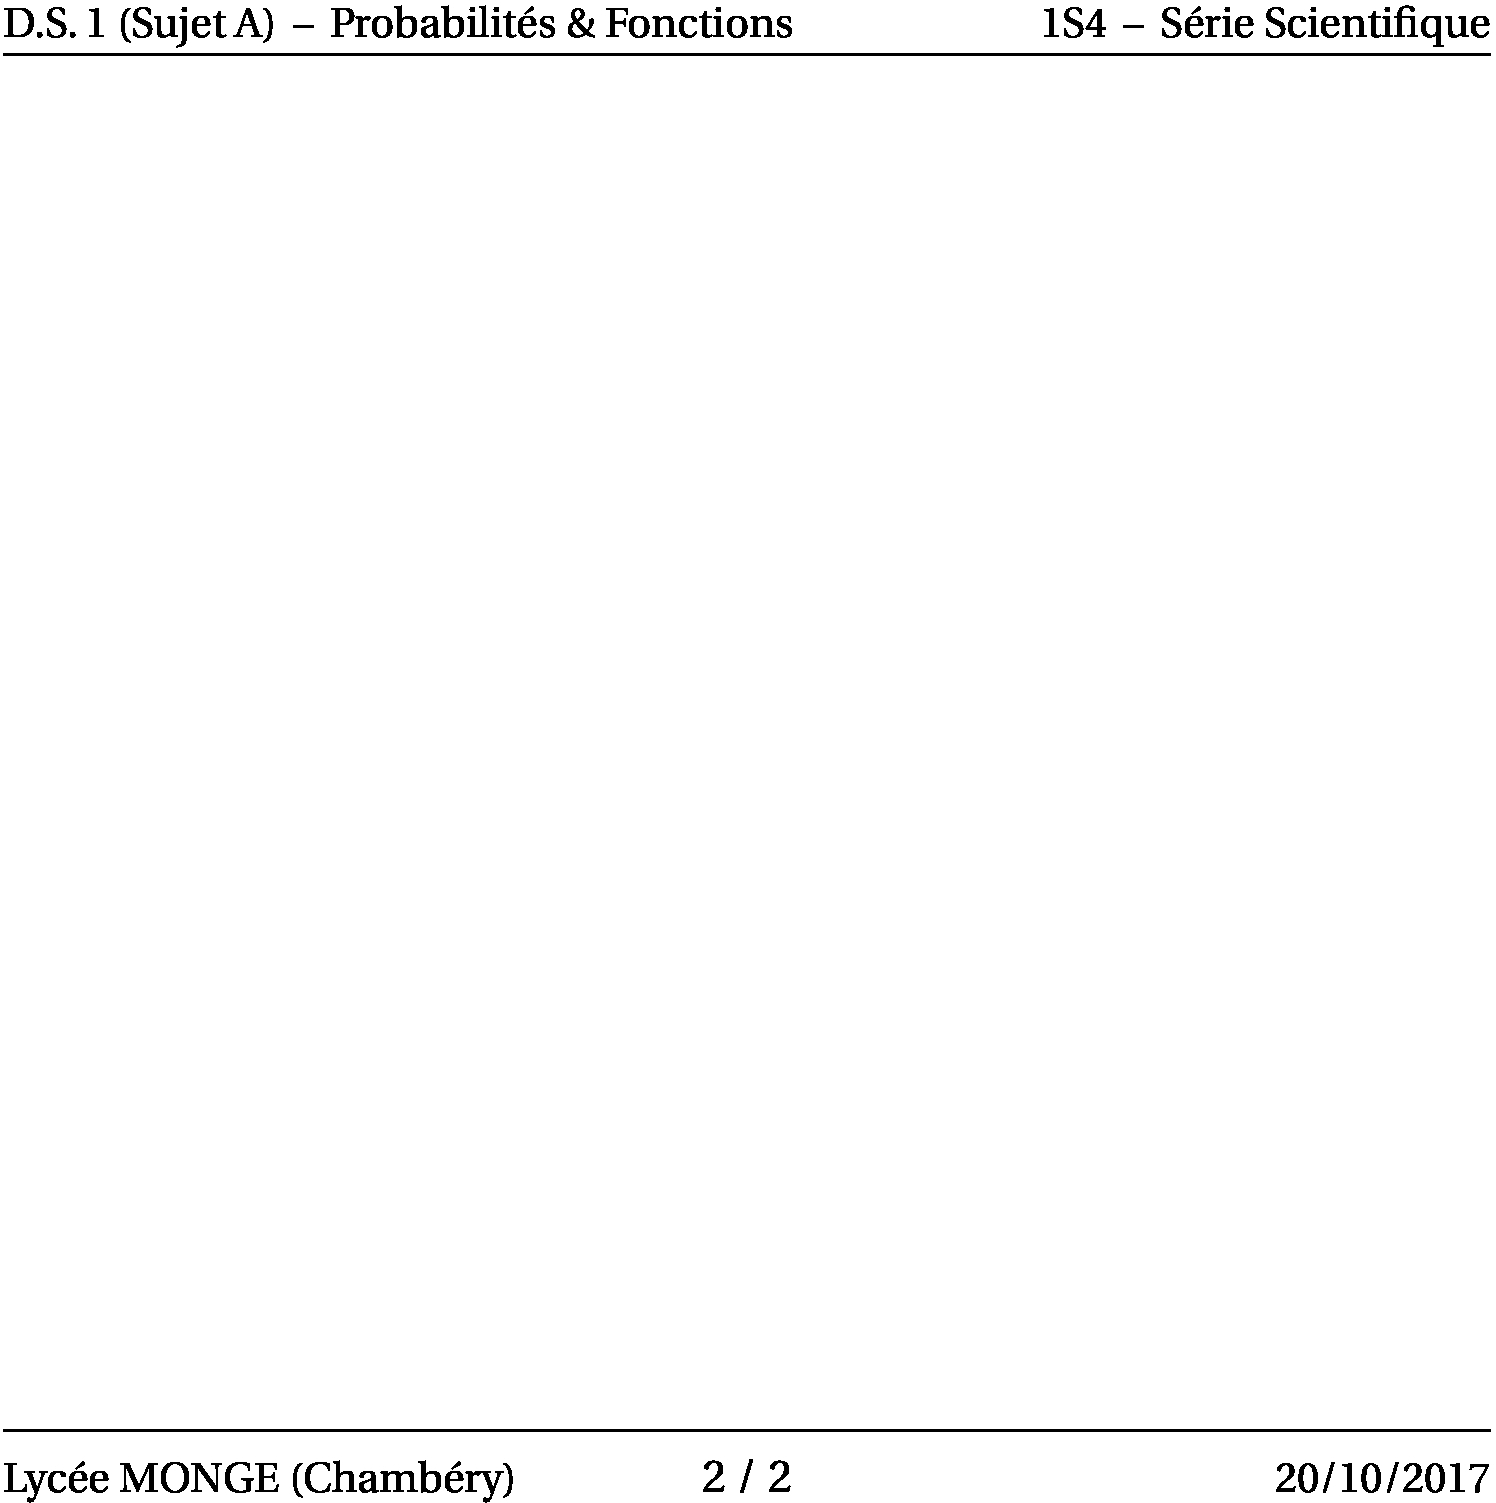
\includegraphics[width=0.43\linewidth]{example-doc[fr]-1.jpg}}
  \caption{Style par défaut.}
  \label{style:default}
\end{figure}

Expliquons maintenant en détail le rôle de chacun des paramètres qui sont tous optionnels. Lorsqu'aucune valeur par défaut n'est indiquée, c'est que cette valeur est un texte vide.

\begin{enumerate}
    \item \verb+deliver+, valant \verb+no+ par défaut, est pour un sujet à rendre avec la copie.
    \begin{itemize}
        \setlength\itemsep{0em}

        \item On peut indiquer \verb+deliver = short+ où \emph{"short"} signifie \emph{"court"}. Ceci affichera une "petite" capsule où l'étudiant renseignera son prénom et son nom. Idéal pour le format \verb+A4+.

        \item Avec \verb+deliver = long+, la capsule sera plus grande. Idéal pour le format \verb+A5+.

        \item Ne pas utiliser l'option revient à passer par \verb+deliver = no+.
    \end{itemize}

    \item \verb+kind+, valant \verb+Test+ par défaut, est le type de devoir : un \emph{"D.S."}, un \emph{"D.M."}, une \emph{"Interrogation Surprise"}, une \emph{"Fiche d'entraînement"}, une \emph{"Activité"}...
    Vous noterez que le terme \emph{"devoir"} ne se limite pas juste aux devoirs notés.

    \item \verb+nb+ est le numéro du devoir.

    \item \verb+subnb+ permet d'indiquer une sorte de numérotation secondaire. C'est utile par exemple pour indiquer \emph{"Sujet A"}, \emph{"Sujet B"} ...

    \item \verb+subject+ permet si besoin de donner la thématique générale du devoir comme par exemple \emph{"Mathématiques"}, \emph{"Informatique Générale"}...

    \item \verb+theme+ sert à compléter la thématique générale en indiquant un ou des points particuliers comme par exemple \emph{"Probabilités"}, \emph{"Réseaux"} ...

    \item \verb+sector+ sert à indiquer une section, au sens administratif, à laquelle s'adresse le devoir. Par exemple, pour un sujet de Baccalauréat S en France, on serait amené à utiliser \verb+sector = Série Scientifique+.

    \item \verb+class+ indique la classe et/ou le groupe auquel est destiné le devoir.

    \item \verb+location+ vous permet d'indiquer un lieu géographique, typiquement un établissement scolaire ou universitaire.

    \item \verb+date+ est pour la date du devoir.

    \item \verb+time+ est pour la durée du devoir.
\end{enumerate}


%    \subsection{Différentes mises en forme}
%
%Le package est fourni avec des exemples de fichiers \LaTeX{} afin d'observer ce que permet \verb+lyxam+. Explorez-les !


    \subsection{Fiche technique}

\IDmacro{exam}{11}{}

\IDkey{kind} le type de devoir, la valeur par défaut étant \verb+Test+.

\IDkey{deliver} pour un sujet à rendre, ou non, avec une zone pour le nom et le prénom de l'étudiant. Trois valeurs possibles : \verb+no+, valeur par défaut, \verb+long+ et \verb+short+.

\IDkey{nb} le numéro du devoir.

\IDkey{subnb} une numérotation secondaire du devoir.

\IDkey{subject} la matière, le sujet du devoir.

\IDkey{theme} un sous-thème ou une sous-partie de la matière ou du sujet du devoir.

\IDkey{sector} un secteur, une section, au sens administratif, à laquelle s'adresse le devoir.

\IDkey{class} la classe concernée par le devoir.

\IDkey{location} le lieu géographique où a lieu le devoir.

\IDkey{date} le texte donnant la date du devoir.

\IDkey{time} le texte indiquant juste la durée du devoir.

\end{document}
